\section{Algorytm rozpoznawania znaków}\label{sec:ocr}
Segmentacja obrazu prowadzi do wyodrębnienia z obrazu żądanych obiektów. Zwykle jest ona pierwszym etapem analizy całego obrazu. Odnalezione obiekty bardzo często poddawane są analizie w celu identyfikacji lub podjęcia decyzji.
\paragraph{}
W przypadku problemu rozpoznawania znaków, zadaniem algorytmu segmentacji jest określenie lokalizacji każdego znaku oraz binaryzacja fragmentów obrazu zawierającego tekst. Kolejnym krokiem jest dostarczenie serii wykadrowanych obrazów binarnych zawierających pojedyncze znaki do algorytmu rozpoznawania znaków. Zadaniem algorytmu rozpoznawania znaków jest określenie, jaki znak tekstu znajduje się na zadanym obrazie.
\paragraph{}
Poniżej zostanie opisanych kilka algorytmów rozpoznawania znaków.
\subsection{Cechy geometryczne}
Zestaw cech geometrycznych jest unikalny dla każdego znaku, dlatego sprawdzając odpowiednie warunki, można określić jego dokładne znaczenie. Właściwości geometryczne znaków zostały obszernie opisane w publikacji \cite{frey91}. Poniżej znajduje się lista wybranych cech geometrycznych, które mogą być brane pod uwagę podczas rozpoznawania znaków.
\begin{itemize}
  \item wysokość oraz szerokość prostokąta otaczającego znak
  \item stosunek liczby punktów należących do znaku do liczby punktów stanowiących tło
  \item stosunek liczby punktów należących do znaku i znajdujących się w górnej połówce obrazu, do liczby punktów należących do znaku i znajdujących się w dolnej połówce obrazu
    \item stosunek liczby punktów należących do znaku i znajdujących się w lewej połówce  obrazu, do liczby punktów należących do znaku i znajdujących się w prawej połówce obrazu
    \item liczba pionowych oraz poziomych krawędzi znaku
\end{itemize}
\subsection{Rzut jasności obiektu}
Metoda rzutu jasności obiektu została opisana na stronie~\pageref{ssec:rzut_jasnosci}. W pierwszej kolejności należy przeskalować obraz do rozmiarów obrazu wzorcowego, a następnie wykonać algorytm rzutu jasności zarówno w pionie, jak i w poziomie. Otrzymane rzuty zostają następnie poddane analizie podobieństwa z rzutami wykonanymi dla znaków wzorcowych. Analiza podobieństwa polega na porównaniu wartości tablic rzutu jasności na poszczególnych indeksach dla obrazu wzorcowego oraz dla obrazu badanego. \\
Na rysunku~\ref{fig:rzut_jasnosci_ocr} przedstawione zostały wzorce kilku znaków, oraz przykładowy obraz wejściowy.

\begin{figure}
  \centering
  \begin{subfigure}[b]{0.42\textwidth}
    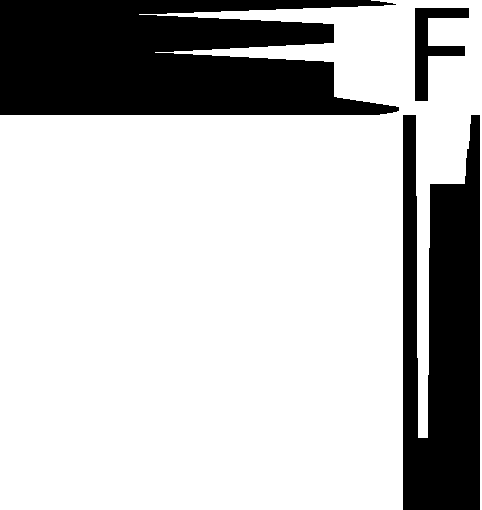
\includegraphics[width=\textwidth]{img/rzut-wzorzec-F}
    \caption{Wzorzec dla litery F}
    \label{fig:rzut_wzorzec_F}
  \end{subfigure}
  ~
  \begin{subfigure}[b]{0.42\textwidth}
    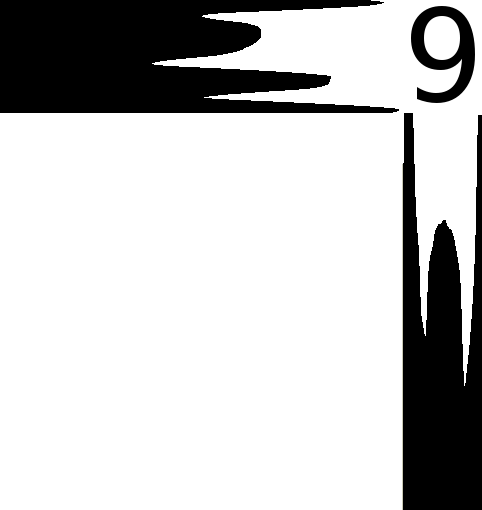
\includegraphics[width=\textwidth]{img/rzut-wzorzec-9}
    \caption{Wzorzec dla cyfry 9}
    \label{fig:rzut_wzorzec_9}
  \end{subfigure}
  \begin{subfigure}[b]{0.44\textwidth}
    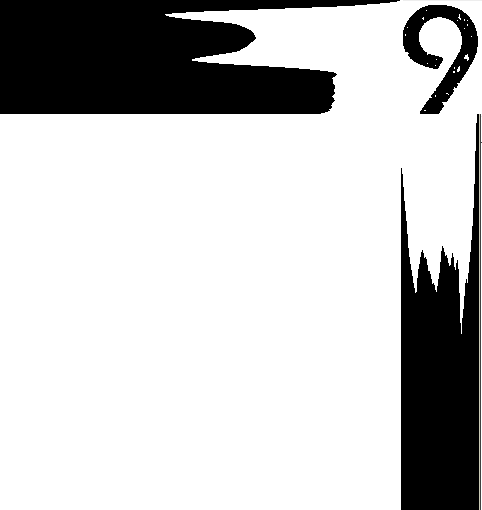
\includegraphics[width=\textwidth]{img/rzut-in-9}
    \caption{Obraz wejściowy, zawierający cyfrę 9}
    \label{fig:rzut_in_9}
  \end{subfigure}
  \caption{Porównanie rzutu jasności dla wybranych znaków}
    \label{fig:rzut_jasnosci_ocr}
\end{figure}

\subsection{Sztuczne sieci neuronowe}
Sztuczne sieci neuronowe(SSN) to struktury tworzone na podobieństwo biologicznych sieci neuronowych \cite{tadeusiewicz93}. SSN mają zdolność do uogólniania zdobytej wiedzy. Podobnie jak w przypadku biologicznych, w sztucznych sieciach neuronowych podstawowym elementem są neurony, które połączone są miedzy sobą za pomocą synaps. Każda synapsa posiada parametr zwany wagą, który jest modyfikowany w poszczególnych fazach uczenia sieci neuronowej. Sieci neuronowe zorganizowane są w strukturze wielowarstwowej:
\begin{itemize}
  \item warstwa wejściowa,
  \item warstwy ukryte,
  \item warstwa wyjściowa.
\end{itemize}
W zależności od złożoności problemu, sieć neuronowa może zawierać różną liczbę neuronów w każdej warstwie, oraz różną liczbę warstw ukrytych. \\
Sztuczne sieci neuronowe można wykorzystać do rozwiązywania problemu rozpoznawania znaków, wykonując najpierw proces uczenia sieci, czyli zadawania na wejście sieci danych uczących wraz z podawaniem poprawnych odpowiedzi. Sieć automatycznie poprawia wagi poszczególnych synaps w taki sposób, aby następna iteracja uczenia zwróciła lepszy wynik. W zależności od struktury sieci, proces ten może wymagać wielu iteracji. Po wykonaniu procesu uczenia, sieć powinna być zdolna samodzielnie rozpoznawać znaki zadane na wejściu.

